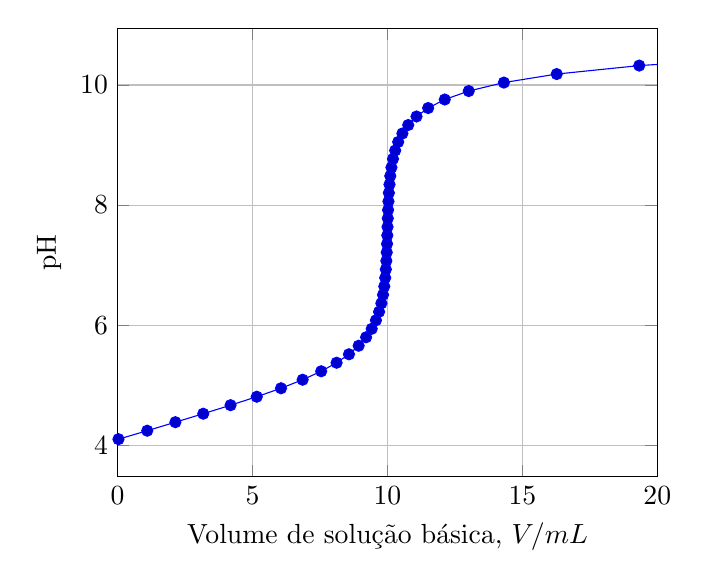
\begin{tikzpicture}
    \begin{axis}
        [
            grid = major,
            xlabel = {Volume de solução básica, $V/\unit{mL}$},
            ylabel = {$\mathrm{pH}$},
            xmin=0, xmax=20,
        ]
    \addplot coordinates
        {
            (0.031, 4.101)
			(1.097, 4.242)
			(2.140, 4.384)
			(3.173, 4.525)
			(4.185, 4.667)
			(5.156, 4.808)
			(6.055, 4.949)
			(6.856, 5.091)
			(7.544, 5.232)
			(8.115, 5.374)
			(8.573, 5.515)
			(8.932, 5.657)
			(9.208, 5.798)
			(9.417, 5.939)
			(9.573, 6.081)
			(9.689, 6.222)
			(9.774, 6.364)
			(9.836, 6.505)
			(9.882, 6.646)
			(9.916, 6.788)
			(9.940, 6.929)
			(9.959, 7.071)
			(9.973, 7.212)
			(9.984, 7.354)
			(9.994, 7.495)
			(10.003, 7.636)
			(10.012, 7.778)
			(10.023, 7.919)
			(10.036, 8.061)
			(10.052, 8.202)
			(10.075, 8.343)
			(10.105, 8.485)
			(10.147, 8.626)
			(10.205, 8.768)
			(10.286, 8.909)
			(10.397, 9.051)
			(10.553, 9.192)
			(10.770, 9.333)
			(11.076, 9.475)
			(11.508, 9.616)
			(12.124, 9.758)
			(13.012, 9.899)
			(14.315, 10.040)
			(16.273, 10.182)
			(19.331, 10.323)
			(24.400, 10.465)
			(33.695, 10.606)   
        };
    \end{axis}
\end{tikzpicture}
